\documentclass{article}
\usepackage{blindtext}
\usepackage{booktabs}
\usepackage[margin=0.25in]{geometry}
\usepackage{subcaption}
\usepackage{graphicx}
\usepackage{caption}
\usepackage{hyperref}
\usepackage{pdflscape}
\usepackage{tikz}
\usepackage{threeparttable}
\usepackage{algorithmic}
\usepackage{tabularx}
\usepackage{amsmath}

\title{Final Ref Comments}

\begin{document}
\maketitle
\tableofcontents
{\footnotesize 
\listoffigures
\listoftables}
\clearpage



\section*{Dependent Variable Specifications}


\clearpage
\begin{table}
\footnotesize
\centering
\caption{Main Table}
\begin{threeparttable}
\footnotesize
 \begin{tabularx}{\textwidth}{l*{5}{>{\centering\arraybackslash}X}} \toprule \setlength{\tabcolsep}{15pt}
&\multicolumn{1}{c}{C. Goodman}&\multicolumn{3}{c}{Census of Governments}&\multicolumn{1}{c}{Census}\\\cmidrule(lr){2-2}\cmidrule(lr){3-5}\cmidrule(lr){6-6}
&\multicolumn{2}{c}{Municipalities}&\multicolumn{1}{c}{School districts}&\multicolumn{1}{c}{Special Districts}&\multicolumn{1}{c}{Main City Share}\\\cmidrule(lr){2-3}\cmidrule(lr){4-4}\cmidrule(lr){5-5}\cmidrule(lr){6-6}
&\multicolumn{1}{c}{(1)}&\multicolumn{1}{c}{(2)}&\multicolumn{1}{c}{(3)}&\multicolumn{1}{c}{(4)}&\multicolumn{1}{c}{(5)}\\
\cmidrule(lr){1-6}
\multicolumn{5}{l}{Panel A: First Stage}\\
\cmidrule(lr){1-6}
$\widehat{GM}$  &    1.771***&    1.771***&    1.841***&    1.771***&    1.771***\\
                &  (0.315)   &  (0.315)   &  (0.330)   &  (0.315)   &  (0.315)   \\
\cmidrule(lr){1-6}
\multicolumn{5}{l}{Panel B: OLS 1940-1970}\\
\cmidrule(lr){1-6}
GM              &    0.003   &    0.005   &    0.101   &   -0.006   &   -0.896***\\
                &  (0.003)   &  (0.004)   &  (0.077)   &  (0.009)   &  (0.171)   \\
\cmidrule(lr){1-6}
\multicolumn{5}{l}{Panel C: 2SLS 1940-1970}\\
\cmidrule(lr){1-6}
GM              &    0.008***&    0.011***&    0.177** &    0.011*  &   -1.577***\\
                &  (0.003)   &  (0.003)   &  (0.072)   &  (0.006)   &  (0.090)   \\
\midrule
1940-70 Avg.    &    -0.26   &    -0.33   &   -12.95   &     0.64   &    -3.37   \\
\cmidrule(lr){1-6}
\multicolumn{5}{l}{Panel D: OLS 1940-2010}\\
\cmidrule(lr){1-6}
GM              &    0.005   &    0.007   &    0.101   &   -0.009   &   -1.137***\\
                &  (0.005)   &  (0.005)   &  (0.077)   &  (0.008)   &  (0.223)   \\
\cmidrule(lr){1-6}
\multicolumn{5}{l}{Panel E: 2SLS 1940-2010}\\
\cmidrule(lr){1-6}
GM              &    0.010***&    0.012***&    0.178** &    0.020***&   -1.873***\\
                &  (0.003)   &  (0.004)   &  (0.073)   &  (0.006)   &  (0.130)   \\
\cmidrule(lr){1-6}
1940-2010 Avg.  &    -0.39   &    -0.49   &   -13.31   &     1.04   &    -7.96   \\
1940 Avg.       &     1.49   &     1.61   &    14.09   &     0.89   &    32.86   \\
First State F-Stat&    31.55   &    31.55   &    31.18   &    31.55   &    31.55   \\
Observations    &     1207   &     1207   &     1201   &     1207   &     1207   \\
 \bottomrule \end{tabularx}

\end{threeparttable}
\label{tab:log_effect}
\end{table}
\clearpage

\clearpage
\begin{table}
\footnotesize
\centering
\caption{Ref Request 1: Log Differences}
\begin{threeparttable}
\footnotesize
 \begin{tabularx}{\textwidth}{l*{5}{>{\centering\arraybackslash}X}} \toprule \setlength{\tabcolsep}{15pt}
&\multicolumn{1}{c}{C. Goodman}&\multicolumn{3}{c}{Census of Governments}&\multicolumn{1}{c}{Census}\\\cmidrule(lr){2-2}\cmidrule(lr){3-5}\cmidrule(lr){6-6}
&\multicolumn{2}{c}{Municipalities}&\multicolumn{1}{c}{School districts}&\multicolumn{1}{c}{Special Districts}&\multicolumn{1}{c}{Main City Share}\\\cmidrule(lr){2-3}\cmidrule(lr){4-4}\cmidrule(lr){5-5}\cmidrule(lr){6-6}
&\multicolumn{1}{c}{(1)}&\multicolumn{1}{c}{(2)}&\multicolumn{1}{c}{(3)}&\multicolumn{1}{c}{(4)}&\multicolumn{1}{c}{(5)}\\
\cmidrule(lr){1-6}
\multicolumn{5}{l}{Panel A: First Stage}\\
\cmidrule(lr){1-6}
$\hat{GM}$      &    1.766***&    1.766***&    1.843***&    1.755***&    1.766***\\
                &  (0.317)   &  (0.317)   &  (0.332)   &  (0.328)   &  (0.317)   \\
\cmidrule(lr){1-6}
\multicolumn{5}{l}{Panel B: OLS 1940-1970}\\
\cmidrule(lr){1-6}
GM              &    0.003   &    0.005   &    0.006   &    0.003   &   -0.000***\\
                &  (0.003)   &  (0.003)   &  (0.017)   &  (0.021)   &  (0.000)   \\
\cmidrule(lr){1-6}
\multicolumn{5}{l}{Panel C: 2SLS 1940-1970}\\
\cmidrule(lr){1-6}
GM              &    0.001   &    0.005   &   -0.031***&    0.002   &   -0.000***\\
                &  (0.003)   &  (0.003)   &  (0.009)   &  (0.007)   &  (0.000)   \\
\midrule
1940-70 Avg.    &     0.13   &     0.08   &    -1.80   &     1.15   &     0.00   \\
\cmidrule(lr){1-6}
\multicolumn{5}{l}{Panel D: OLS 1940-2010}\\
\cmidrule(lr){1-6}
GM              &    0.003   &    0.000   &    0.003   &   -0.018   &   -0.000***\\
                &  (0.003)   &  (0.005)   &  (0.017)   &  (0.018)   &  (0.000)   \\
\cmidrule(lr){1-6}
\multicolumn{5}{l}{Panel E: 2SLS 1940-2010}\\
\cmidrule(lr){1-6}
GM              &   -0.001   &    0.000   &   -0.036***&   -0.023** &   -0.001***\\
                &  (0.003)   &  (0.004)   &  (0.010)   &  (0.011)   &  (0.000)   \\
\cmidrule(lr){1-6}
1940-2010 Avg.  &     0.18   &     0.12   &    -1.92   &     1.71   &     0.00   \\
1940 Avg.       &     1.48   &     1.61   &    14.05   &     0.88   &    32.78   \\
First Stage F-Stat&    31.08   &    31.08   &    30.84   &    28.68   &    31.08   \\
Observations    &      130   &      130   &      118   &      114   &      130   \\
 \bottomrule \end{tabularx}

\end{threeparttable}
\label{tab:log_effect}
\end{table}
\clearpage

\clearpage
\begin{table}
\footnotesize
\centering
\caption{Ref Request 1: Log Differences + popgrowth control}
\begin{threeparttable}
\footnotesize
 \begin{tabularx}{\textwidth}{l*{5}{>{\centering\arraybackslash}X}} \toprule \setlength{\tabcolsep}{15pt}
&\multicolumn{1}{c}{C. Goodman}&\multicolumn{3}{c}{Census of Governments}&\multicolumn{1}{c}{Census}\\\cmidrule(lr){2-2}\cmidrule(lr){3-5}\cmidrule(lr){6-6}
&\multicolumn{2}{c}{Municipalities}&\multicolumn{1}{c}{School districts}&\multicolumn{1}{c}{Special Districts}&\multicolumn{1}{c}{Main City Share}\\\cmidrule(lr){2-3}\cmidrule(lr){4-4}\cmidrule(lr){5-5}\cmidrule(lr){6-6}
&\multicolumn{1}{c}{(1)}&\multicolumn{1}{c}{(2)}&\multicolumn{1}{c}{(3)}&\multicolumn{1}{c}{(4)}&\multicolumn{1}{c}{(5)}\\
\cmidrule(lr){1-6}
\multicolumn{5}{l}{Panel A: First Stage}\\
\cmidrule(lr){1-6}
$\hat{GM}$      &    1.865***&    1.865***&    1.939***&    1.852***&    1.865***\\
                &  (0.319)   &  (0.319)   &  (0.339)   &  (0.331)   &  (0.319)   \\
\cmidrule(lr){1-6}
\multicolumn{5}{l}{Panel B: OLS 1940-1970}\\
\cmidrule(lr){1-6}
GM              &    0.003   &    0.005   &    0.006   &    0.004   &   -0.017***\\
                &  (0.003)   &  (0.003)   &  (0.017)   &  (0.021)   &  (0.006)   \\
\cmidrule(lr){1-6}
\multicolumn{5}{l}{Panel C: 2SLS 1940-1970}\\
\cmidrule(lr){1-6}
GM              &    0.004** &    0.007** &   -0.023** &    0.003   &   -0.030***\\
                &  (0.002)   &  (0.003)   &  (0.009)   &  (0.007)   &  (0.002)   \\
\midrule
1940-70 Avg.    &     0.13   &     0.08   &    -1.80   &     1.15   &     0.27   \\
\cmidrule(lr){1-6}
\multicolumn{5}{l}{Panel D: OLS 1940-2010}\\
\cmidrule(lr){1-6}
GM              &    0.003   &    0.000   &    0.003   &   -0.018   &   -0.035***\\
                &  (0.003)   &  (0.005)   &  (0.017)   &  (0.018)   &  (0.009)   \\
\cmidrule(lr){1-6}
\multicolumn{5}{l}{Panel E: 2SLS 1940-2010}\\
\cmidrule(lr){1-6}
GM              &    0.004   &    0.004   &   -0.028***&   -0.017*  &   -0.054***\\
                &  (0.003)   &  (0.004)   &  (0.010)   &  (0.010)   &  (0.004)   \\
\cmidrule(lr){1-6}
1940-2010 Avg.  &     0.18   &     0.12   &    -1.92   &     1.71   &     0.30   \\
1940 Avg.       &     1.48   &     1.61   &    14.08   &     0.88   &  3282.25   \\
First Stage F-Stat&    34.18   &    34.18   &    32.73   &    31.39   &    34.18   \\
Observations    &      130   &      130   &      118   &      114   &      130   \\
 \bottomrule \end{tabularx}

\end{threeparttable}
\label{tab:log_effect}
\end{table}
\clearpage

\clearpage
\begin{table}
\footnotesize
\centering
\caption{Ref Request 2: Pct Outcome}
\begin{threeparttable}
\footnotesize
 \begin{tabularx}{\textwidth}{l*{5}{>{\centering\arraybackslash}X}} \toprule \setlength{\tabcolsep}{15pt}
&\multicolumn{1}{c}{C. Goodman}&\multicolumn{3}{c}{Census of Governments}&\multicolumn{1}{c}{Census}\\\cmidrule(lr){2-2}\cmidrule(lr){3-5}\cmidrule(lr){6-6}
&\multicolumn{2}{c}{Municipalities}&\multicolumn{1}{c}{School districts}&\multicolumn{1}{c}{Special Districts}&\multicolumn{1}{c}{Main City Share}\\\cmidrule(lr){2-3}\cmidrule(lr){4-4}\cmidrule(lr){5-5}\cmidrule(lr){6-6}
&\multicolumn{1}{c}{(1)}&\multicolumn{1}{c}{(2)}&\multicolumn{1}{c}{(3)}&\multicolumn{1}{c}{(4)}&\multicolumn{1}{c}{(5)}\\
\cmidrule(lr){1-6}
\multicolumn{5}{l}{Panel A: First Stage}\\
\cmidrule(lr){1-6}
$\hat{GM}$      &    1.771***&    1.771***&    1.842***&    1.771***&    1.771***\\
                &  (0.315)   &  (0.315)   &  (0.330)   &  (0.315)   &  (0.315)   \\
\cmidrule(lr){1-6}
\multicolumn{5}{l}{Panel B: OLS 1940-1970}\\
\cmidrule(lr){1-6}
GM              &   -0.000   &    0.002   &    0.097   &   -0.000   & -115.435***\\
                &  (0.002)   &  (0.003)   &  (0.076)   &  (0.015)   & (39.031)   \\
\cmidrule(lr){1-6}
\multicolumn{5}{l}{Panel C: 2SLS 1940-1970}\\
\cmidrule(lr){1-6}
GM              &    0.002   &    0.006** &    0.159** &    0.051***& -313.303***\\
                &  (0.002)   &  (0.002)   &  (0.068)   &  (0.014)   & (35.240)   \\
\midrule
1940-70 Avg.    &     0.16   &     0.11   &   -12.40   &     1.40   &  1722.81   \\
\cmidrule(lr){1-6}
\multicolumn{5}{l}{Panel D: OLS 1940-2010}\\
\cmidrule(lr){1-6}
GM              &   -0.001   &    0.000   &    0.094   &    0.002   & -226.522***\\
                &  (0.003)   &  (0.004)   &  (0.077)   &  (0.023)   & (77.510)   \\
\cmidrule(lr){1-6}
\multicolumn{5}{l}{Panel E: 2SLS 1940-2010}\\
\cmidrule(lr){1-6}
GM              &    0.002   &    0.004   &    0.151** &    0.112***& -663.575***\\
                &  (0.003)   &  (0.003)   &  (0.069)   &  (0.029)   & (99.163)   \\
\cmidrule(lr){1-6}
1940-2010 Avg.  &     0.24   &     0.15   &   -12.66   &     2.87   &  3449.08   \\
1940 Avg.       &     1.48   &     1.61   &    14.08   &     0.88   &  3282.25   \\
First Stage F-Stat&    31.54   &    31.54   &    31.18   &    31.54   &    31.54   \\
Observations    &      130   &      130   &      118   &      130   &      130   \\
 \bottomrule \end{tabularx}

\end{threeparttable}
\label{tab:log_effect}
\end{table}
\clearpage

\clearpage
\begin{table}
\footnotesize
\centering
\caption{Ref Request 2: Pct on Pct}
\begin{threeparttable}
\footnotesize
 \begin{tabularx}{\textwidth}{l*{5}{>{\centering\arraybackslash}X}} \toprule \setlength{\tabcolsep}{15pt}
&\multicolumn{1}{c}{C. Goodman}&\multicolumn{3}{c}{Census of Governments}&\multicolumn{1}{c}{Census}\\\cmidrule(lr){2-2}\cmidrule(lr){3-5}\cmidrule(lr){6-6}
&\multicolumn{2}{c}{Municipalities}&\multicolumn{1}{c}{School districts}&\multicolumn{1}{c}{Special Districts}&\multicolumn{1}{c}{Main City Share}\\\cmidrule(lr){2-3}\cmidrule(lr){4-4}\cmidrule(lr){5-5}\cmidrule(lr){6-6}
&\multicolumn{1}{c}{(1)}&\multicolumn{1}{c}{(2)}&\multicolumn{1}{c}{(3)}&\multicolumn{1}{c}{(4)}&\multicolumn{1}{c}{(5)}\\
\cmidrule(lr){1-6}
\multicolumn{5}{l}{Panel A: First Stage}\\
\cmidrule(lr){1-6}
$\hat{GM}$      &    0.432   &    0.432   &    0.367   &    0.432   &    0.432   \\
                &  (0.294)   &  (0.294)   &  (0.346)   &  (0.294)   &  (0.294)   \\
\cmidrule(lr){1-6}
\multicolumn{5}{l}{Panel B: OLS 1940-1970}\\
\cmidrule(lr){1-6}
Percentage Change in Urban Black Population&   -0.004** &   -0.002   &    0.038   &    0.007   &   58.479   \\
                &  (0.002)   &  (0.002)   &  (0.091)   &  (0.018)   & (54.331)   \\
\cmidrule(lr){1-6}
\multicolumn{5}{l}{Panel C: 2SLS 1940-1970}\\
\cmidrule(lr){1-6}
Percentage Change in Urban Black Population&    0.008   &    0.026** &    0.797   &    0.211** & -1.3e+03***\\
                &  (0.007)   &  (0.011)   &  (0.565)   &  (0.098)   &(482.842)   \\
\midrule
1940-70 Avg.    &     0.16   &     0.11   &   -12.40   &     1.40   &  1722.81   \\
\cmidrule(lr){1-6}
\multicolumn{5}{l}{Panel D: OLS 1940-2010}\\
\cmidrule(lr){1-6}
Percentage Change in Urban Black Population&   -0.006** &   -0.005*  &    0.034   &   -0.002   &  107.667   \\
                &  (0.003)   &  (0.003)   &  (0.092)   &  (0.028)   &(129.110)   \\
\cmidrule(lr){1-6}
\multicolumn{5}{l}{Panel E: 2SLS 1940-2010}\\
\cmidrule(lr){1-6}
Percentage Change in Urban Black Population&    0.006   &    0.016   &    0.759   &    0.459** & -2.7e+03** \\
                &  (0.010)   &  (0.013)   &  (0.552)   &  (0.198)   &(1074.699)   \\
\cmidrule(lr){1-6}
1940-2010 Avg.  &     0.24   &     0.15   &   -12.66   &     2.87   &  3449.08   \\
1940 Avg.       &     1.48   &     1.61   &    14.08   &     0.88   &  3282.25   \\
First Stage F-Stat&     2.15   &     2.15   &     1.13   &     2.15   &     2.15   \\
Observations    &      130   &      130   &      118   &      130   &      130   \\
 \bottomrule \end{tabularx}

\end{threeparttable}
\label{tab:log_effect}
\end{table}
\clearpage


\clearpage
\begin{table}
\footnotesize
\centering
\caption{Raw Differences}
\begin{threeparttable}
\footnotesize
 \begin{tabularx}{\textwidth}{l*{5}{>{\centering\arraybackslash}X}} \toprule \setlength{\tabcolsep}{15pt}
&\multicolumn{1}{c}{C. Goodman}&\multicolumn{3}{c}{Census of Governments}&\multicolumn{1}{c}{Census}\\\cmidrule(lr){2-2}\cmidrule(lr){3-5}\cmidrule(lr){6-6}
&\multicolumn{2}{c}{Municipalities}&\multicolumn{1}{c}{School districts}&\multicolumn{1}{c}{Special Districts}&\multicolumn{1}{c}{Main City Share}\\\cmidrule(lr){2-3}\cmidrule(lr){4-4}\cmidrule(lr){5-5}\cmidrule(lr){6-6}
&\multicolumn{1}{c}{(1)}&\multicolumn{1}{c}{(2)}&\multicolumn{1}{c}{(3)}&\multicolumn{1}{c}{(4)}&\multicolumn{1}{c}{(5)}\\
\cmidrule(lr){1-6}
\multicolumn{5}{l}{Panel A: First Stage}\\
\cmidrule(lr){1-6}
$\hat{GM}$      &    1.771***&    1.771***&    1.842***&    1.771***&    1.771***\\
                &  (0.315)   &  (0.315)   &  (0.330)   &  (0.315)   &  (0.315)   \\
\cmidrule(lr){1-6}
\multicolumn{5}{l}{Panel B: OLS 1940-1970}\\
\cmidrule(lr){1-6}
GM              &    1.148** &    1.103*  &  -16.922** &    8.039*  & -1.5e+04***\\
                &  (0.575)   &  (0.619)   &  (7.465)   &  (4.531)   &(5152.559)   \\
\cmidrule(lr){1-6}
\multicolumn{5}{l}{Panel C: 2SLS 1940-1970}\\
\cmidrule(lr){1-6}
GM              &    1.740***&    1.824***&  -26.682***&    9.481***& -3.4e+04***\\
                &  (0.392)   &  (0.436)   &  (4.893)   &  (1.628)   &(5930.385)   \\
\midrule
1940-70 Avg.    &     7.22   &     5.39   &  -320.96   &    52.42   & 48923.45   \\
\cmidrule(lr){1-6}
\multicolumn{5}{l}{Panel D: OLS 1940-2010}\\
\cmidrule(lr){1-6}
GM              &    1.353*  &    1.027   &  -17.575** &    6.666   & -4.5e+04***\\
                &  (0.774)   &  (0.810)   &  (7.579)   &  (4.188)   &(8692.185)   \\
\cmidrule(lr){1-6}
\multicolumn{5}{l}{Panel E: 2SLS 1940-2010}\\
\cmidrule(lr){1-6}
GM              &    1.821***&    1.839***&  -27.567***&   14.356***& -7.8e+04***\\
                &  (0.590)   &  (0.630)   &  (4.987)   &  (2.209)   &(1.1e+04)   \\
\cmidrule(lr){1-6}
1940-2010 Avg.  &    10.34   &     7.67   &  -327.23   &    93.10   & 64430.39   \\
1940 Avg.       &     1.48   &     1.61   &    14.08   &     0.88   &  3282.25   \\
First Stage F-Stat&    31.54   &    31.54   &    31.18   &    31.54   &    31.54   \\
Observations    &      130   &      130   &      118   &      130   &      130   \\
 \bottomrule \end{tabularx}

\end{threeparttable}
\label{tab:log_effect}
\end{table}
\clearpage


\clearpage
\begin{table}
\footnotesize
\centering
\caption{1970 P.C. Outcome}
\begin{threeparttable}
\footnotesize
 \begin{tabularx}{\textwidth}{l*{5}{>{\centering\arraybackslash}X}} \toprule \setlength{\tabcolsep}{15pt}
&\multicolumn{1}{c}{C. Goodman}&\multicolumn{3}{c}{Census of Governments}&\multicolumn{1}{c}{Census}\\\cmidrule(lr){2-2}\cmidrule(lr){3-5}\cmidrule(lr){6-6}
&\multicolumn{2}{c}{Municipalities}&\multicolumn{1}{c}{School districts}&\multicolumn{1}{c}{Special Districts}&\multicolumn{1}{c}{Main City Share}\\\cmidrule(lr){2-3}\cmidrule(lr){4-4}\cmidrule(lr){5-5}\cmidrule(lr){6-6}
&\multicolumn{1}{c}{(1)}&\multicolumn{1}{c}{(2)}&\multicolumn{1}{c}{(3)}&\multicolumn{1}{c}{(4)}&\multicolumn{1}{c}{(5)}\\
\cmidrule(lr){1-6}
\multicolumn{5}{l}{Panel A: First Stage}\\
\cmidrule(lr){1-6}
$\hat{GM}$      &    1.762***&    1.762***&    1.824***&    1.788***&    1.648***\\
                &  (0.310)   &  (0.308)   &  (0.336)   &  (0.321)   &  (0.328)   \\
\cmidrule(lr){1-6}
\multicolumn{5}{l}{Panel B: OLS 1940-1970}\\
\cmidrule(lr){1-6}
GM              &    0.002   &    0.003   &   -0.001   &   -0.005   &  -71.272***\\
                &  (0.002)   &  (0.003)   &  (0.004)   &  (0.009)   & (17.313)   \\
\cmidrule(lr){1-6}
\multicolumn{5}{l}{Panel C: 2SLS 1940-1970}\\
\cmidrule(lr){1-6}
GM              &    0.012***&    0.015***&    0.005   &    0.053***& -136.271***\\
                &  (0.004)   &  (0.004)   &  (0.004)   &  (0.014)   &  (9.157)   \\
\midrule
1940-70 Avg.    &     1.22   &     1.28   &     1.13   &     1.52   &  2946.69   \\
\cmidrule(lr){1-6}
\multicolumn{5}{l}{Panel D: OLS 1940-2010}\\
\cmidrule(lr){1-6}
GM              &    0.004   &    0.004   &   -0.003   &   -0.007   &  -81.939***\\
                &  (0.004)   &  (0.004)   &  (0.003)   &  (0.009)   & (15.204)   \\
\cmidrule(lr){1-6}
\multicolumn{5}{l}{Panel E: 2SLS 1940-2010}\\
\cmidrule(lr){1-6}
GM              &    0.014***&    0.015***&    0.005** &    0.066***& -143.265***\\
                &  (0.004)   &  (0.005)   &  (0.002)   &  (0.012)   &  (9.955)   \\
\cmidrule(lr){1-6}
1940-2010 Avg.  &     1.09   &     1.13   &     0.78   &     1.93   &  2489.56   \\
1940 Avg.       &     1.48   &     1.61   &    14.08   &     0.88   &  3282.25   \\
First Stage F-Stat&    32.26   &    32.74   &    29.42   &    30.99   &    25.27   \\
Observations    &      130   &      130   &      118   &      130   &      130   \\
 \bottomrule \end{tabularx}

\end{threeparttable}
\label{tab:log_effect}
\end{table}
\clearpage

\clearpage
\begin{table}
\footnotesize
\centering
\caption{1970 Outcome}
\begin{threeparttable}
\footnotesize
 \begin{tabularx}{\textwidth}{l*{5}{>{\centering\arraybackslash}X}} \toprule \setlength{\tabcolsep}{15pt}
&\multicolumn{1}{c}{C. Goodman}&\multicolumn{3}{c}{Census of Governments}&\multicolumn{1}{c}{Census}\\\cmidrule(lr){2-2}\cmidrule(lr){3-5}\cmidrule(lr){6-6}
&\multicolumn{2}{c}{Municipalities}&\multicolumn{1}{c}{School districts}&\multicolumn{1}{c}{Special Districts}&\multicolumn{1}{c}{Main City Share}\\\cmidrule(lr){2-3}\cmidrule(lr){4-4}\cmidrule(lr){5-5}\cmidrule(lr){6-6}
&\multicolumn{1}{c}{(1)}&\multicolumn{1}{c}{(2)}&\multicolumn{1}{c}{(3)}&\multicolumn{1}{c}{(4)}&\multicolumn{1}{c}{(5)}\\
\cmidrule(lr){1-6}
\multicolumn{5}{l}{Panel A: First Stage}\\
\cmidrule(lr){1-6}
$\hat{GM}$      &    1.389***&    1.380***&    1.589***&    1.620***&    1.755***\\
                &  (0.306)   &  (0.302)   &  (0.287)   &  (0.306)   &  (0.307)   \\
\cmidrule(lr){1-6}
\multicolumn{5}{l}{Panel B: OLS 1940-1970}\\
\cmidrule(lr){1-6}
Percentage Point Change in Urban Black Population&   -0.276   &   -0.325   &    6.248** &    5.808   & -166.062***\\
                &  (0.546)   &  (0.620)   &  (2.609)   &  (4.044)   & (51.660)   \\
\cmidrule(lr){1-6}
\multicolumn{5}{l}{Panel C: 2SLS 1940-1970}\\
\cmidrule(lr){1-6}
Percentage Point Change in Urban Black Population&    5.470***&    5.920***&    3.570** &   10.832***& -393.757***\\
                &  (0.835)   &  (0.856)   &  (1.558)   &  (2.046)   & (54.579)   \\
\midrule
1940-70 Avg.    &    56.38   &    58.35   &    57.94   &    83.74   &  3103.12   \\
\cmidrule(lr){1-6}
\multicolumn{5}{l}{Panel D: OLS 1940-2010}\\
\cmidrule(lr){1-6}
Percentage Point Change in Urban Black Population&   -0.564   &   -0.654   &    6.031** &    3.252   & -464.433***\\
                &  (0.828)   &  (0.882)   &  (2.439)   &  (2.809)   & (97.816)   \\
\cmidrule(lr){1-6}
\multicolumn{5}{l}{Panel E: 2SLS 1940-2010}\\
\cmidrule(lr){1-6}
Percentage Point Change in Urban Black Population&    5.428***&    5.738***&    2.918** &   15.204***& -833.043***\\
                &  (0.985)   &  (0.985)   &  (1.481)   &  (2.597)   &(102.807)   \\
\cmidrule(lr){1-6}
1940-2010 Avg.  &    59.25   &    60.63   &    51.67   &   124.42   &  3258.19   \\
1940 Avg.       &     1.48   &     1.61   &    14.05   &     0.88   &    32.78   \\
First Stage F-Stat&    20.56   &    20.84   &    30.67   &    28.10   &    32.75   \\
Observations    &      130   &      130   &      118   &      130   &      130   \\
 \bottomrule \end{tabularx}

\end{threeparttable}
\label{tab:log_effect}
\end{table}
\clearpage

\clearpage
\begin{table}
\footnotesize
\centering
\caption{1970 Outcome, Popgrowth Control}
\begin{threeparttable}
\footnotesize
 \begin{tabularx}{\textwidth}{l*{5}{>{\centering\arraybackslash}X}} \toprule \setlength{\tabcolsep}{15pt}
&\multicolumn{1}{c}{C. Goodman}&\multicolumn{3}{c}{Census of Governments}&\multicolumn{1}{c}{Census}\\\cmidrule(lr){2-2}\cmidrule(lr){3-5}\cmidrule(lr){6-6}
&\multicolumn{2}{c}{Municipalities}&\multicolumn{1}{c}{School districts}&\multicolumn{1}{c}{Special Districts}&\multicolumn{1}{c}{Main City Share}\\\cmidrule(lr){2-3}\cmidrule(lr){4-4}\cmidrule(lr){5-5}\cmidrule(lr){6-6}
&\multicolumn{1}{c}{(1)}&\multicolumn{1}{c}{(2)}&\multicolumn{1}{c}{(3)}&\multicolumn{1}{c}{(4)}&\multicolumn{1}{c}{(5)}\\
\cmidrule(lr){1-6}
\multicolumn{5}{l}{Panel A: First Stage}\\
\cmidrule(lr){1-6}
$\hat{GM}$      &    1.493***&    1.470***&    1.667***&    1.718***&    1.851***\\
                &  (0.313)   &  (0.306)   &  (0.295)   &  (0.305)   &  (0.308)   \\
\cmidrule(lr){1-6}
\multicolumn{5}{l}{Panel B: OLS 1940-1970}\\
\cmidrule(lr){1-6}
GM              &   -0.244   &   -0.342   &    6.320** &    5.996   & -1.7e+04***\\
                &  (0.570)   &  (0.626)   &  (2.474)   &  (4.050)   &(4595.081)   \\
\cmidrule(lr){1-6}
\multicolumn{5}{l}{Panel C: 2SLS 1940-1970}\\
\cmidrule(lr){1-6}
GM              &    5.388***&    5.830***&    4.554***&   10.001***& -3.3e+04***\\
                &  (0.820)   &  (0.847)   &  (1.442)   &  (1.967)   &(4682.853)   \\
\midrule
1940-70 Avg.    &    56.09   &    58.35   &    57.94   &    83.74   &310000.00   \\
\cmidrule(lr){1-6}
\multicolumn{5}{l}{Panel D: OLS 1940-2010}\\
\cmidrule(lr){1-6}
GM              &   -0.531   &   -0.678   &    6.111***&    3.251   & -4.7e+04***\\
                &  (0.856)   &  (0.897)   &  (2.292)   &  (2.802)   &(9230.720)   \\
\cmidrule(lr){1-6}
\multicolumn{5}{l}{Panel E: 2SLS 1940-2010}\\
\cmidrule(lr){1-6}
GM              &    5.435***&    5.701***&    3.954***&   14.940***& -7.1e+04***\\
                &  (0.966)   &  (0.971)   &  (1.355)   &  (2.555)   &(8702.952)   \\
\cmidrule(lr){1-6}
1940-2010 Avg.  &    59.21   &    60.63   &    51.67   &   124.42   &330000.00   \\
1940 Avg.       &     1.48   &     1.61   &    14.08   &     0.88   &  3282.25   \\
First Stage F-Stat&    22.69   &    23.13   &    31.82   &    31.62   &    36.03   \\
Observations    &      130   &      130   &      118   &      130   &      130   \\
 \bottomrule \end{tabularx}

\end{threeparttable}
\label{tab:log_effect}
\end{table}
\clearpage


\clearpage
\begin{table}
\footnotesize
\centering
\caption{Poisson}
\begin{threeparttable}
\footnotesize
 \begin{tabularx}{\textwidth}{l*{4}{>{\centering\arraybackslash}X}} \toprule \setlength{\tabcolsep}{15pt}
&\multicolumn{1}{c}{C. Goodman}&\multicolumn{3}{c}{Census of Governments}\\\cmidrule(lr){2-2}\cmidrule(lr){3-5}
&\multicolumn{2}{c}{Municipalities}&\multicolumn{1}{c}{School districts}&\multicolumn{1}{c}{Special Districts}\\\cmidrule(lr){2-3}\cmidrule(lr){4-4}\cmidrule(lr){5-5}
&\multicolumn{1}{c}{(1)}&\multicolumn{1}{c}{(2)}&\multicolumn{1}{c}{(3)}&\multicolumn{1}{c}{(4)}\\
\cmidrule(lr){1-5}
\multicolumn{4}{l}{Panel A: First Stage}\\
\cmidrule(lr){1-5}
$\hat{GM}$      &    1.398***&    1.377***&    1.587***&    1.623***\\
                &  (0.308)   &  (0.300)   &  (0.283)   &  (0.305)   \\
\cmidrule(lr){1-5}
\multicolumn{4}{l}{Panel B: OLS 1940-1970}\\
\cmidrule(lr){1-5}
GM              &    0.016***&    0.016** &    0.052***&    0.039*  \\
                &  (0.006)   &  (0.006)   &  (0.018)   &  (0.021)   \\
\cmidrule(lr){1-5}
\multicolumn{4}{l}{Panel C: 2SLS 1940-1970}\\
\cmidrule(lr){1-5}
GM              &    0.012   &    0.012   &    0.003   &    0.039   \\
                &  (0.011)   &  (0.011)   &  (0.025)   &  (0.034)   \\
\midrule
1940-70 Avg.    &     7.22   &     5.39   &  -320.96   &    52.42   \\
\cmidrule(lr){1-5}
\multicolumn{4}{l}{Panel D: OLS 1940-2010}\\
\cmidrule(lr){1-5}
GM              &    0.015** &    0.013*  &    0.052***&    0.016   \\
                &  (0.007)   &  (0.007)   &  (0.017)   &  (0.012)   \\
\cmidrule(lr){1-5}
\multicolumn{4}{l}{Panel E: 2SLS 1940-2010}\\
\cmidrule(lr){1-5}
GM              &    0.010   &    0.012   &    0.002   &    0.039   \\
                &  (0.013)   &  (0.013)   &  (0.024)   &  (0.025)   \\
\cmidrule(lr){1-5}
1940-2010 Avg.  &    10.34   &     7.67   &  -327.23   &    93.10   \\
1940 Avg.       &    48.87   &    52.96   &   381.55   &    31.32   \\
First Stage F-Stat&    20.57   &    20.99   &    31.51   &    28.40   \\
Observations    &      130   &      130   &      117   &      130   \\
 \bottomrule \end{tabularx}

\end{threeparttable}
\label{tab:log_effect}
\end{table}
\clearpage

\clearpage
\begin{table}
\footnotesize
\centering
\caption{Poisson, popgrowth control}
\begin{threeparttable}
\footnotesize
 \begin{tabularx}{\textwidth}{l*{4}{>{\centering\arraybackslash}X}} \toprule \setlength{\tabcolsep}{15pt}
&\multicolumn{1}{c}{C. Goodman}&\multicolumn{3}{c}{Census of Governments}\\\cmidrule(lr){2-2}\cmidrule(lr){3-5}
&\multicolumn{2}{c}{Municipalities}&\multicolumn{1}{c}{School districts}&\multicolumn{1}{c}{Special Districts}\\\cmidrule(lr){2-3}\cmidrule(lr){4-4}\cmidrule(lr){5-5}
&\multicolumn{1}{c}{(1)}&\multicolumn{1}{c}{(2)}&\multicolumn{1}{c}{(3)}&\multicolumn{1}{c}{(4)}\\
\cmidrule(lr){1-5}
\multicolumn{4}{l}{Panel A: First Stage}\\
\cmidrule(lr){1-5}
$\hat{GM}$      &    1.493***&    1.470***&    1.667***&    1.718***\\
                &  (0.313)   &  (0.306)   &  (0.294)   &  (0.305)   \\
\cmidrule(lr){1-5}
\multicolumn{4}{l}{Panel B: OLS 1940-1970}\\
\cmidrule(lr){1-5}
GM              &    0.016***&    0.016***&    0.054***&    0.038*  \\
                &  (0.006)   &  (0.006)   &  (0.016)   &  (0.021)   \\
\cmidrule(lr){1-5}
\multicolumn{4}{l}{Panel C: 2SLS 1940-1970}\\
\cmidrule(lr){1-5}
GM              &    0.016*  &    0.017*  &    0.011   &    0.032   \\
                &  (0.010)   &  (0.010)   &  (0.023)   &  (0.031)   \\
\midrule
1940-70 Avg.    &     7.22   &     5.39   &  -320.96   &    52.42   \\
\cmidrule(lr){1-5}
\multicolumn{4}{l}{Panel D: OLS 1940-2010}\\
\cmidrule(lr){1-5}
GM              &    0.014** &    0.013*  &    0.055***&    0.016   \\
                &  (0.007)   &  (0.007)   &  (0.015)   &  (0.012)   \\
\cmidrule(lr){1-5}
\multicolumn{4}{l}{Panel E: 2SLS 1940-2010}\\
\cmidrule(lr){1-5}
GM              &    0.016   &    0.017   &    0.011   &    0.042*  \\
                &  (0.012)   &  (0.011)   &  (0.022)   &  (0.024)   \\
\cmidrule(lr){1-5}
1940-2010 Avg.  &    10.34   &     7.67   &  -327.23   &    93.10   \\
1940 Avg.       &    48.87   &    52.96   &   381.55   &    31.32   \\
First Stage F-Stat&    22.69   &    23.13   &    32.10   &    31.62   \\
Observations    &      130   &      130   &      117   &      130   \\
 \bottomrule \end{tabularx}

\end{threeparttable}
\label{tab:log_effect}
\end{table}
\clearpage

\clearpage
\begin{table}
\footnotesize
\centering
\caption{Poisson, 1970 Population exposure}
\begin{threeparttable}
\footnotesize
 \begin{tabularx}{\textwidth}{l*{4}{>{\centering\arraybackslash}X}} \toprule \setlength{\tabcolsep}{15pt}
&\multicolumn{1}{c}{C. Goodman}&\multicolumn{3}{c}{Census of Governments}\\\cmidrule(lr){2-2}\cmidrule(lr){3-5}
&\multicolumn{2}{c}{Municipalities}&\multicolumn{1}{c}{School districts}&\multicolumn{1}{c}{Special Districts}\\\cmidrule(lr){2-3}\cmidrule(lr){4-4}\cmidrule(lr){5-5}
&\multicolumn{1}{c}{(1)}&\multicolumn{1}{c}{(2)}&\multicolumn{1}{c}{(3)}&\multicolumn{1}{c}{(4)}\\
\cmidrule(lr){1-5}
\multicolumn{4}{l}{Panel A: First Stage}\\
\cmidrule(lr){1-5}
$\hat{GM}$      &    1.736***&    1.735***&    1.859***&    1.794***\\
                &  (0.321)   &  (0.325)   &  (0.348)   &  (0.326)   \\
\cmidrule(lr){1-5}
\multicolumn{4}{l}{Panel B: OLS 1940-1970}\\
\cmidrule(lr){1-5}
GM              &    0.003   &    0.005   &    0.010   &    0.018   \\
                &  (0.004)   &  (0.005)   &  (0.008)   &  (0.015)   \\
\cmidrule(lr){1-5}
\multicolumn{4}{l}{Panel C: 2SLS 1940-1970}\\
\cmidrule(lr){1-5}
GM              &    0.012** &    0.015***&   -0.008   &    0.036   \\
                &  (0.005)   &  (0.005)   &  (0.014)   &  (0.026)   \\
\midrule
1940-70 Avg.    &     7.25   &     5.39   &  -320.96   &    52.42   \\
\cmidrule(lr){1-5}
\multicolumn{4}{l}{Panel D: OLS 1940-2010}\\
\cmidrule(lr){1-5}
GM              &    0.007   &    0.008   &    0.012   &   -0.001   \\
                &  (0.006)   &  (0.007)   &  (0.008)   &  (0.009)   \\
\cmidrule(lr){1-5}
\multicolumn{4}{l}{Panel E: 2SLS 1940-2010}\\
\cmidrule(lr){1-5}
GM              &    0.017** &    0.020** &   -0.002   &    0.026*  \\
                &  (0.008)   &  (0.008)   &  (0.011)   &  (0.013)   \\
\cmidrule(lr){1-5}
1940-2010 Avg.  &    10.12   &     7.67   &  -327.23   &    93.10   \\
1940 Avg.       &    49.14   &    52.96   &   381.55   &    31.32   \\
First Stage F-Stat&    29.20   &    28.58   &    28.60   &    30.24   \\
Observations    &      130   &      130   &      117   &      130   \\
 \bottomrule \end{tabularx}

\end{threeparttable}
\label{tab:log_effect}
\end{table}
\clearpage


\section*{Event Studies}
\clearpage
\begin{figure}
	\centering
	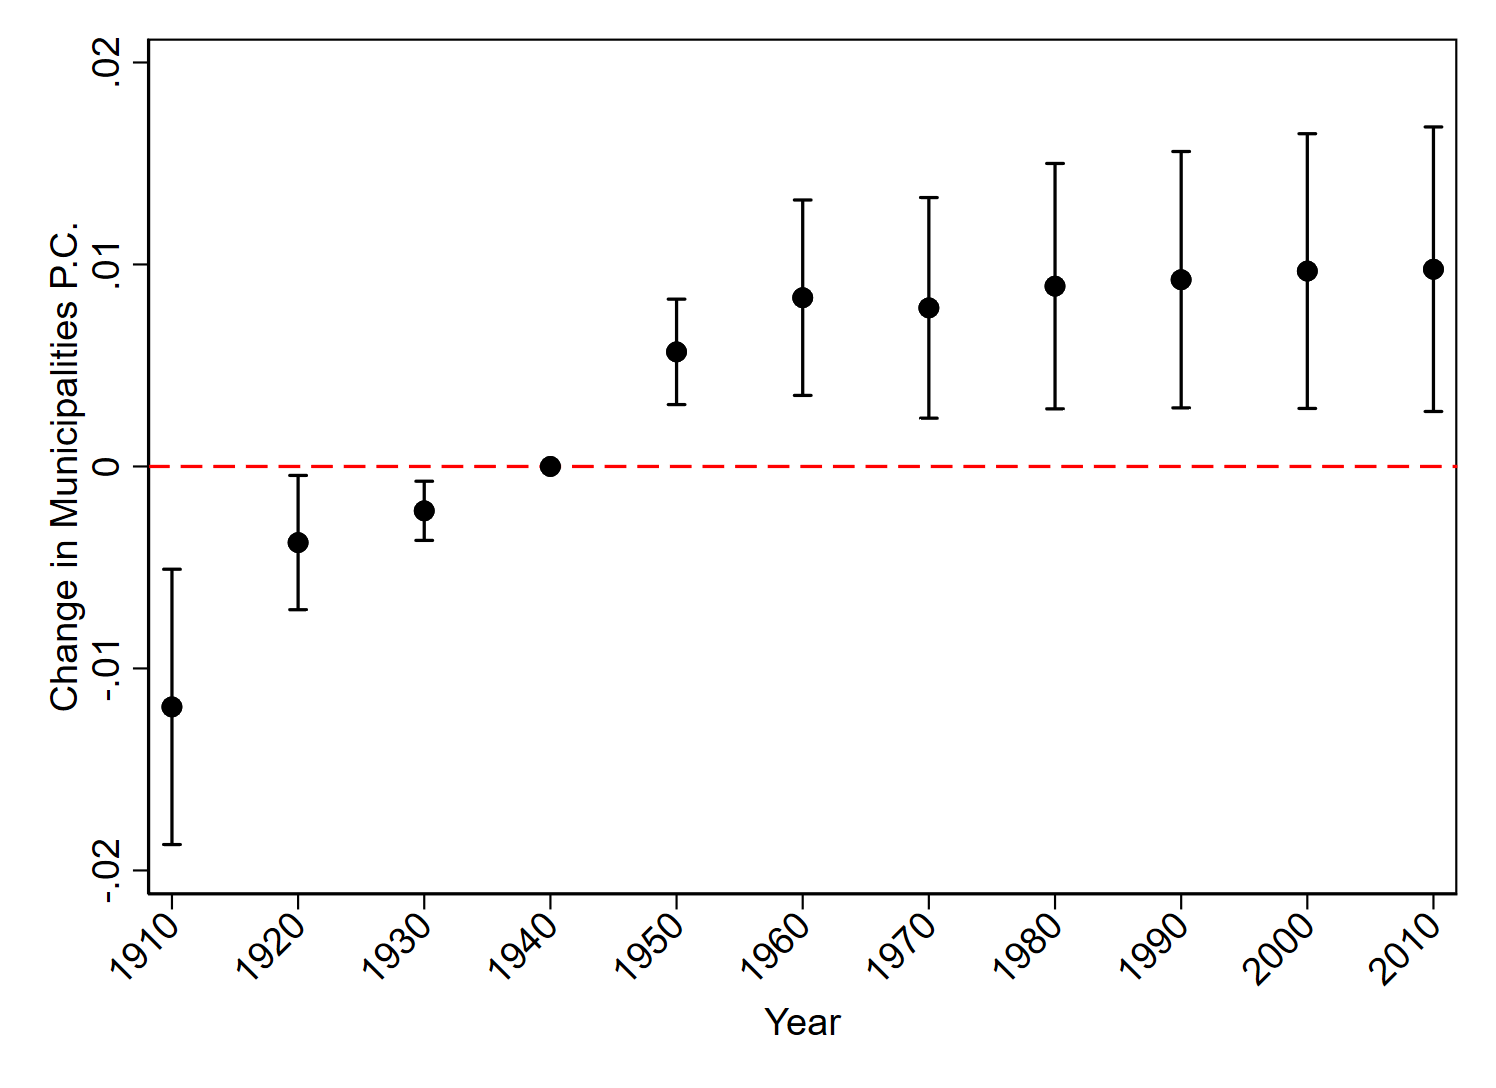
\includegraphics[width=0.7\textwidth]{figures/RR3/es_ssaggregate_nhgis_full_6.png}
	\caption{1940 Imbalanced Controls}
\end{figure}
\clearpage
\begin{figure}
	\centering
	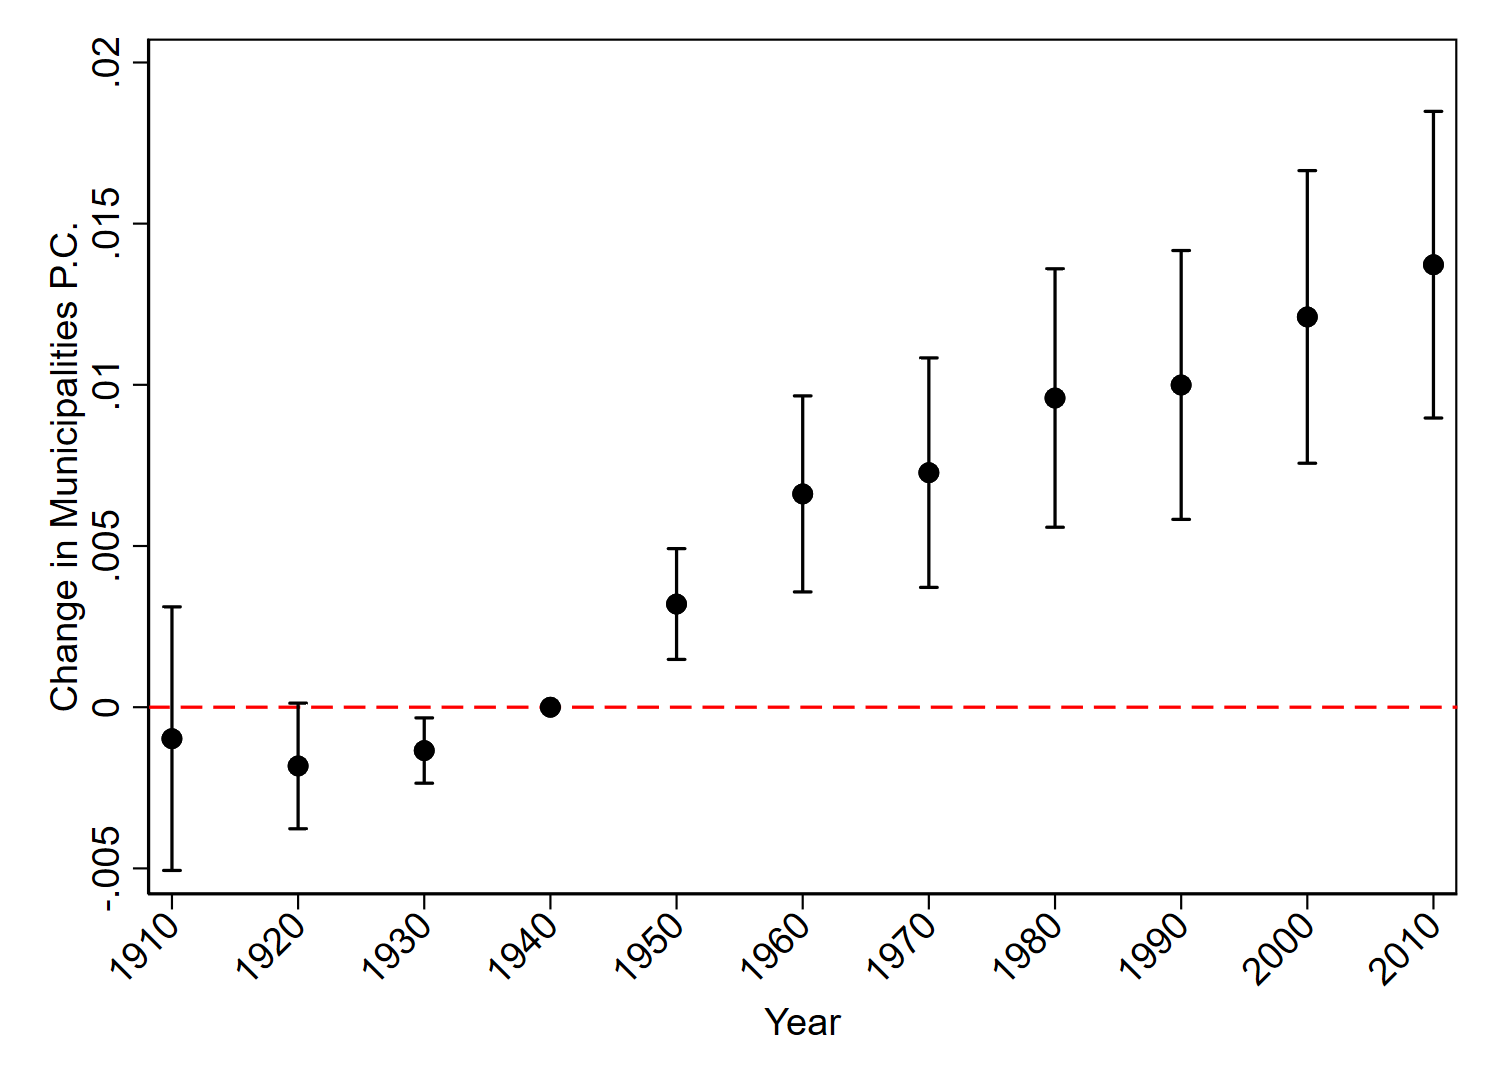
\includegraphics[width=0.7\textwidth]{figures/RR3/es_ssaggregate_nhgis_full_2.png}
	\caption{Baseline Controls}
\end{figure}
\clearpage
\begin{figure}
	\centering
	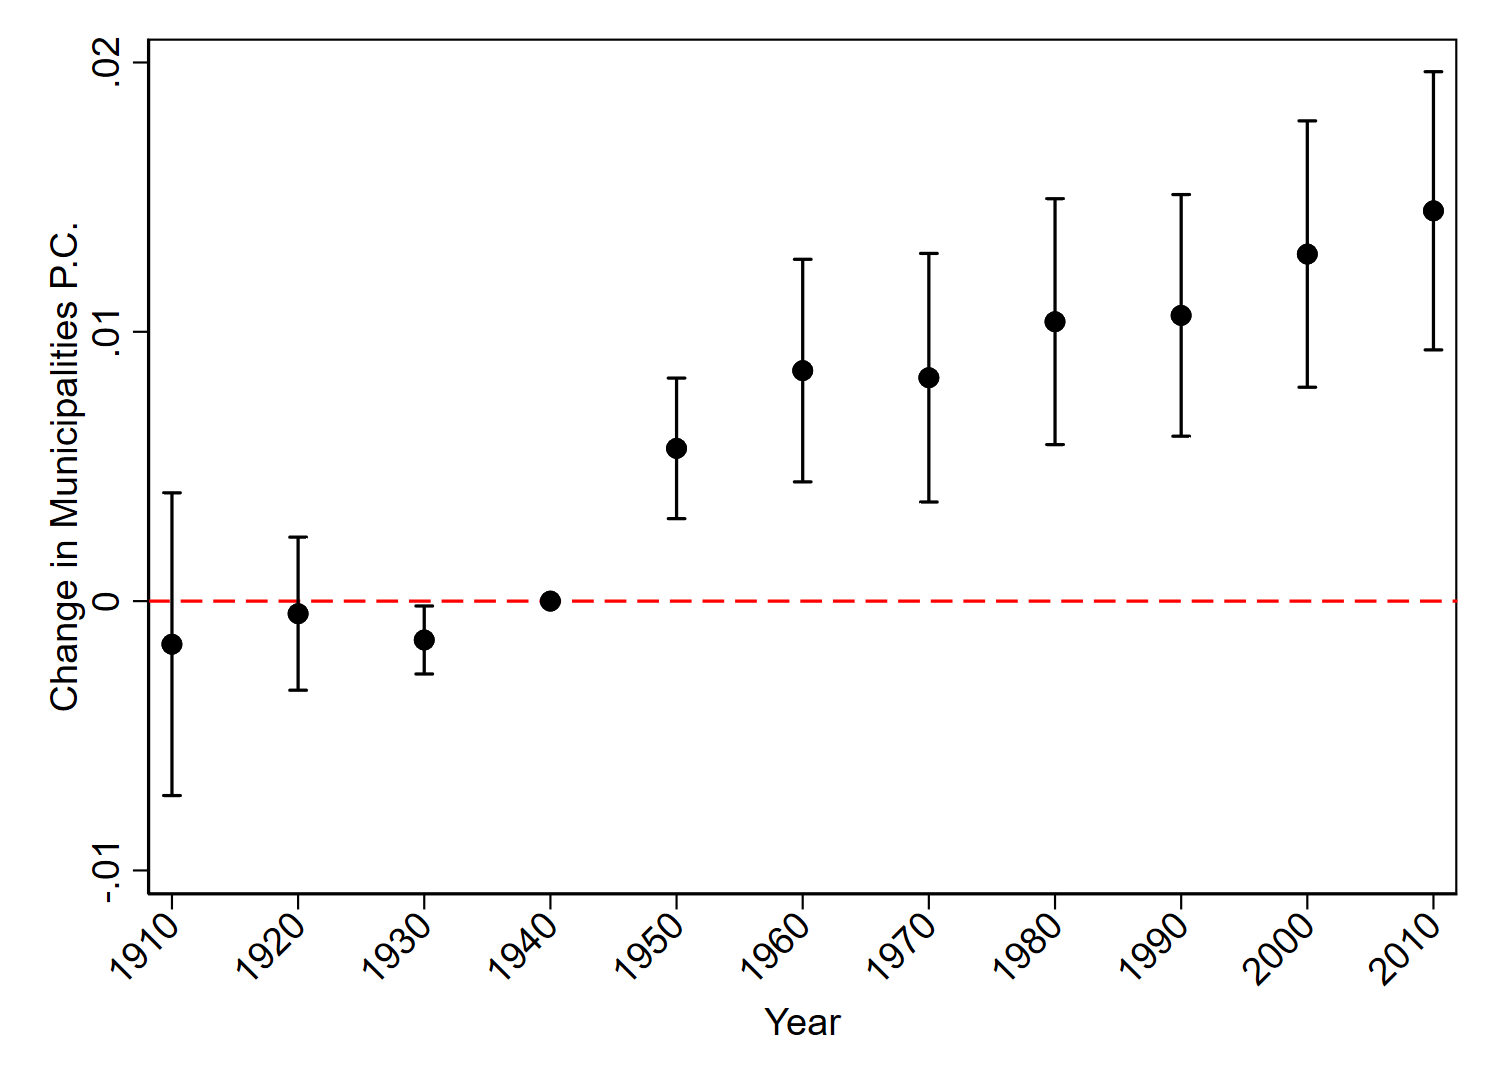
\includegraphics[width=0.7\textwidth]{figures/RR3/es_ssaggregate_nhgis_full_4.png}
	\caption{1940 Mean Income, Lab. Force. Mfg and Popdens Varying}
\end{figure}
\clearpage
\begin{figure}
	\centering
	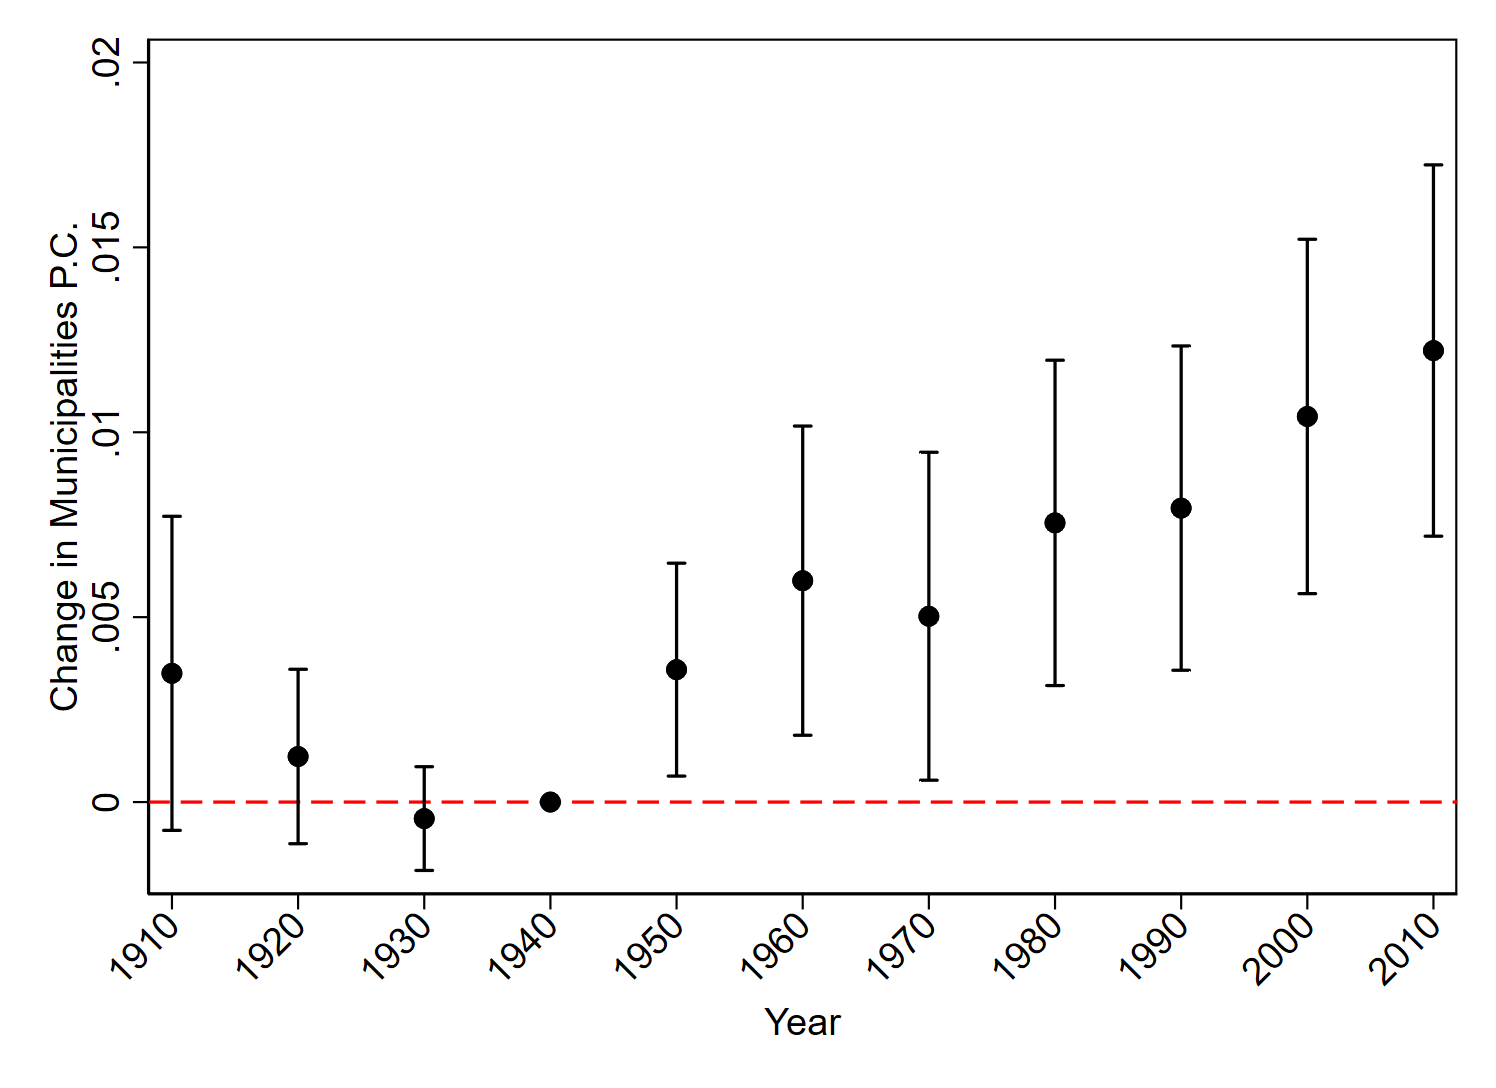
\includegraphics[width=0.7\textwidth]{figures/RR3/es_ssaggregate_nhgis_full_8.png}
	\caption{Lab. Force. Mfg and Popdens Varying}
\end{figure}
\end{document}
